\documentclass[./\jobname.tex]{subfiles}
\begin{document}

\chapter{Experimental Design}
This chapter serves as an introduction to the experiments and gives an overview on how these are conducted. An integral part of solver comparison is to define a testbed that holds example problems with a known analytical solution. Further, quality measurements must be defined that compares the numerical to the analytical solution. The baseline for all experiments is the \gls{fem} solver NGSolve (\cite{mitchell_nist_2018}).

\section{Testbed}
The testbed is a collection of multiple different 2-dimensional scalar \gls{pde}s that are analytically solved such that $u(\mathbf{x}): \mathbf{R}^2 \rightarrow \mathbf{R}$ is a solution to the underlaying PDE. These can be used to demonstrate the correct implementation of a solver. The testbed can also be used to compare the performance of the classical \gls{fem} solver (NGSolve) with the \gls{ci} solver. The actual equations are displayed in the appendix \ref{chap:testbed}. The equations used here are a mixture of multiple different testbeds. Specifically, the equations 2 and 3 are picked from the testbed in \cite{chaquet_using_2019}. These problems were also used by \cite{tsoulos_solving_2006} and \cite{panagant_solving_2014}. Preliminary tests have shown that the equations used in these paper are rather simple to approximate. Thus, more complicate equations are added to test the solvability over a wider variety of functions. The more complicated equations are taken from the National Institute of Standards and Technology (NIST) website (\cite{mitchell_nist_2018}) that provides benchmarking problems for \gls{fem} slovers with adaptive mesh refinement methods. The other equations 0A, 0B and 8 are specially created to show different properties of the solver. 

\textbf{PDE 0A: Gauss Kernel (equation \ref{eq:pde0a})} The analytic solution of this problem can be approximated arbitrarely close, since the solution is a sum of 5 different Gauss kernels. \todo{link Gauss kernel equations} The purpose of this PDE is to show that the algorithm converges. \\

\textbf{PDE 0B: GSin Kernel (equation \ref{eq:pde0b})} Similar to the PDE 0A, this problem is a sum of GSin kernels. To keep the search dimensionality roughly the same as in PDE 0A, the problem can be solved with 3 kernels. \todo{link Gsin chapter here} Again, the purpose of this equation is to determine the convergence with other kernel.  \\

\textbf{PDE 1: Polynomial 2D (equation \ref{eq:pde1})} The solution of this equation is a polynomial of order 20. The function is 0 on the boundary of the unit square. (\cite{mitchell_nist_2018}) \\

\textbf{PDE 2: Chaquet PDE 1 (equation \ref{eq:pde2})} This is the problem of the Chaquet testbed, that is also used by several other authors. Its main purpose is to build the bridge to those papers so that the results can be compared. \cite{chaquet_using_2019} \\

\textbf{PDE 3: Chaquet PDE 3 (equation \ref{eq:pde3})} This equation is solved by a polynomial of order 2. Again, the purpose is to compare the results to other papers. \cite{chaquet_using_2019} \\

\textbf{PDE 4: Sine Bump 2D (equation \ref{eq:pde4})} The sine bump occures in a similar fashion in both, the Chaquet testbed (PDE 8 in \cite{chaquet_using_2019}) as well as the NIST (\cite{mitchell_nist_2018}) testbed. This means that the underlying solution function is the same, but the \gls{pde} is posed differently. Preliminary results have shown that the formulation of the NIST testbed is harder to solve. Thus, the formulation of Chaquet is disregarded and the NIST problem is implemented. \\

\textbf{PDE 5: Arctan Circular Wave Front (equation \ref{eq:pde5})} The main difficulty of this problem is the transition from the flat plateaus to the steep gradient of the circular wave front. Preliminary test have shown that this equation is one of the hardest in this testbed. (\cite{mitchell_nist_2018})\\

\textbf{PDE 6: Peak 2D (equation \ref{eq:pde6})} The solution to this problem is described by a single Gaussian ``peak'' at $(0.5, 0.5)$ with a large exponent. This solution could be approximated by a single Gaussian kernel. The difficulty here is the steep gradient and a small region of interest. (\cite{mitchell_nist_2018})\\

\textbf{PDE 7: Boundary Line Singularity (equation \ref{eq:pde7})} This equation is only determined on $x \in \mathbf{R}^{+}$, which results in a singularity line at $x = 0$. Towards this line the gradient increases.  (\cite{mitchell_nist_2018})\\

\textbf{PDE 8: Interior Point Singularity (equation \ref{eq:pde8})} The idea of this \gls{pde} is similar to the problem 7, but the singularity is located on the inner domain. The solution to this problem is not defined at $(0.5, 0.5)$, resulting in a very hard problem. \\

\textbf{PDE 9: Arctan Wave Front Homogeneous Boundary Conditions 2D (equation \ref{eq:pde9})} Similar to \gls{pde} 5, the difficulty of this problem is the steep gradient. Additionaly, the boundary condition is zero wich results in sharp corners on the boundary, that are hard to approximate. (\cite{mitchell_nist_2018})\\


\section{Software Architecture}

\definecolor{light-gray}{gray}{0.9}

\definecolor{testbed_colour}{RGB}{255,153,51}
\definecolor{opt_algo_colour}{RGB}{204,0,0}
\definecolor{kernels_colour}{RGB}{0,127,255}
\definecolor{post_proc_colour}{RGB}{198,41,255}

To simplify the preparation, execution and evaluation of the experiments, a comprehensive software architecture is defined. The \gls{uml} class diagram can be seen in the appendix \ref{chap:software_architecture}. The architecture is organised in 4 main segments. 

\textcolor{opt_algo_colour}{\large \underline{\textbf{optimisation algorithm in red}}} \\
The \colorbox{light-gray}{\lstinline[basicstyle=\ttfamily\color{black}]|IOptAlgoBase|} interface must be implemented by every \colorbox{light-gray}{\lstinline[basicstyle=\ttfamily\color{black}]|OptAlgo|} class to ensure the compatibility with \colorbox{light-gray}{\lstinline[basicstyle=\ttfamily\color{black}]|CiPdeBase|} class of the testbed. A nice side-effect is that it reduces the number of user-defined parameters. An optimisation algorithm of this class must only take an initial guess (e.g. the starting population) as well as two stopping criteria: the maximum number of generation or a minimum error to reach. Also a fitness function (i.e. the function to be optimised) must be provided. Four lists of the same length are returned: the optimum-guess, the function value, the crossover probability and the scale factor per each generation. The actual implementation of the algorithm is not predefined. 

\textcolor{kernels_colour}{\large \underline{\textbf{kernels in blue}}} \\
As described in chapter \ref{chap:candidate_rep}, a candidate solution is defined as a sum of radial basis function. In order to test different candidate representations, different classes must be implemented. Again, to ensure compatibility with the \colorbox{light-gray}{\lstinline[basicstyle=\ttfamily\color{black}]|CiPdeBase|} class, all representations must implement the \colorbox{light-gray}{\lstinline[basicstyle=\ttfamily\color{black}]|IKernelBase|} interface. This assures that all classes have a method that can calculate the solution as well as first and second order derivatives. Here, only two kernels are imlemented.

\textcolor{testbed_colour}{\large \underline{\textbf{testbed in orange}}} \\
The testbed holds the 11 differential equations used in all experiments. The testbed is abstraced in such a way that an experiment is as simple as creating an \gls{pde} object and calling its solve method. All testbed classes must implement the \colorbox{light-gray}{\lstinline[basicstyle=\ttfamily\color{black}]|ITestbenchBase|} interface. This ensures the minimal functionality of every subsequent class. Currently two classes implement this interface, the \colorbox{light-gray}{\lstinline[basicstyle=\ttfamily\color{black}]|FemPdeBase|} and the \colorbox{light-gray}{\lstinline[basicstyle=\ttfamily\color{black}]|CiPdeBase|}. These are the base classes that provide the specific attributes and methods needed for the \gls{fem} solver and the \gls{ci} solver. The actual \gls{pde} problems are implemented in the classes \colorbox{light-gray}{\lstinline[basicstyle=\ttfamily\color{black}]|FemPde0|} or \colorbox{light-gray}{\lstinline[basicstyle=\ttfamily\color{black}]|CiPde0|} which inherit from the \colorbox{light-gray}{\lstinline[basicstyle=\ttfamily\color{black}]|FemPdeBase|} and the \colorbox{light-gray}{\lstinline[basicstyle=\ttfamily\color{black}]|CiPdeBase|}, respectively. The number in their name is representative for all different testbench problems and every \gls{pde} has its own class. Since all \gls{pde} classes have the same methods and attributes and only differ in their implementation and name, they do not have to be displayed separately. Therefore, they are symbolised together by a ``stacked notation'' used in the class diagram. Some methods in these classes must be overridden and adapted to the current \gls{pde} problem, which is indicated by the $\land$ character.

\textcolor{post_proc_colour}{\large \underline{\textbf{post processing in purple}}} \\
Although the post processing block is not actually a class, it is still represented in this diagram. This module provides funtions that take \colorbox{light-gray}{\lstinline[basicstyle=\ttfamily\color{black}]|FemPdeN|} or \colorbox{light-gray}{\lstinline[basicstyle=\ttfamily\color{black}]|CiPdeN|} objects and performs actions with them. \todo{update implemented function description}

\begin{itemize}
	\item \colorbox{light-gray}{\lstinline[basicstyle=\ttfamily\color{black}]|bool saveExpObj(obj, path)|} \\
	Save an experiment object as 
	\item \colorbox{light-gray}{\lstinline[basicstyle=\ttfamily\color{black}]|CiPdeBase loadExpObject(path)|} \\
	Load an experiment object
	\item \colorbox{light-gray}{\lstinline[basicstyle=\ttfamily\color{black}]|bool drawGaussKernel(parameter, ggb)|} \\
	Draw Gauss kernel to 
	\item \colorbox{light-gray}{\lstinline[basicstyle=\ttfamily\color{black}]|bool drawGSinKernel(parameter, ggb)|} \\
	Draw Gsin kernel to
\end{itemize}

\section{Metric} 
\label{chap:metric}
In order to scientifically compare the results produced by the different solvers, some metrics are necessary. Three important solver-properties are measured: the execution time, the memory usage and the quality of the numerical solution. The following chapters describe the measurement process in greater detail. 

\subsection{Execution Time}
\label{chap:metric_time}
The solving time is measured within the \colorbox{light-gray}{\lstinline[basicstyle=\ttfamily\color{black}]|solve()|} method of either class. The time module of the \cite{python_standard_library_time_2020} is used to interact with the system clock. The resolution, that the time module can access, depends on the system it is running on. Specifically, on the machine used in all further experiments, \colorbox{light-gray}{\lstinline[basicstyle=\ttfamily\color{black}]|time.time()|} returns a 24 byte float that represents the time passed since 1st of January 1970. Usually, consecutive calls of this function return increasing values - changing the system time could interfere with the correctness of this value.\\ 

As the execution time of a program depends on many other factors, such as the current system load, the CPU temperature and the process scheduler, it is necessary to view it as a random variant. Thus, multiple replications have to be done before trying to interprete the results. These replications are not done within the \colorbox{light-gray}{\lstinline[basicstyle=\ttfamily\color{black}]|solve()|} function and must be applied during the experiment. To reduce the random effects and prevent possible outlier, the Python garbage collector is switched off during the time measurement. For a step-by-step description, the pseudocode is displayed in the appendix \ref{chap:solve_function}. 

\subsection{Memory Usage}
\label{chap:metric_mem}
Similar to the solving time measurement, the memory usage is determined within the \colorbox{light-gray}{\lstinline[basicstyle=\ttfamily\color{black}]|solve()|} method. The psutil module (\cite{rodola_psutil_2020}) provides the functionality to read the amount of memory attached to a process at a given time. The function call \colorbox{light-gray}{\lstinline[basicstyle=\ttfamily\color{black}]|process.memory_info()|} returns a dictionary with multiple indicators about the current state of the process. Of special interest is the \colorbox{light-gray}{\lstinline[basicstyle=\ttfamily\color{black}]|rss|} field. \gls{rss} is the memory that is currently allocated by a process and actually held within the main memory. This means that memory that is currently swapped out, is not regarded with this measurement. Preliminary tests have shown that although the garbage collector was turned off, consecutive calls of \colorbox{light-gray}{\lstinline[basicstyle=\ttfamily\color{black}]|process.memory_info()|} could result in a decreasing amount of rss-memory allocated by the process. A reason for this phenomenon could be that currently allocated memory is swapped out. When evaluating the results, these datapoints must be disregarded or treated as outliers. \\

Without assuming anything about the inner workings of the process, the memory is also a random variant. Thus, similar to the time measurement, replications have to be performed. The same pseudocode as for the time measurement (appendix \ref{chap:solve_function}) also applies here.

\subsection{Quality Measurement}
\label{chap:metric_quality}
Although the fitness function is the criterion that is optimised, it is not applicable as an objective quality measure. As \cite{chaquet_using_2019} describe, it depends on multiple factors:
\begin{itemize}
	\item user-defined parameters $\xi$ and $\phi$ 
	\item the formulation of the \gls{pde} 
	\item number of collocation points used 
	\item number of kernels used
\end{itemize}
Thus, \cite{chaquet_using_2019} define a new quality measurement based on the \gls{rmse} over the collocation points as seen in equation \ref{eq:rmse_chaquet}. 
\begin{equation}
\label{eq:rmse_chaquet}
RMSE^2 = \frac{\sum_{i=1, \mathbf{x}_i \in C}^{n_C} \left|\left| \mathbf{u}(\mathbf{x}_i) - \mathbf{u_{ext}}(\mathbf{x}_i) \right|\right|^2 + \sum_{j=1, \mathbf{x}_j \in B}^{n_B} \left|\left| \mathbf{u}(\mathbf{x}_j) - \mathbf{u_{ext}}(\mathbf{x}_j) \right|\right|^2}{m(n_C + n_B)}
\end{equation}
This quality criterion also three inherent issues. At first, it firmly depends on the number of collocation points used. In an algorithm that uses self-adaptive collocation points, this measurement would be rendered useless. Further, the quality is only measured on the collocation points and not in between. However, a good solution fits not only these discrete points, but the whole domain. Finally, the \gls{fem} method does not know anything about collocation points. A good quality measurement tool only use the numerical and analytical solution, independently of the solving method. \\

This leads to the quality measurement formulation used in this thesis: the L2 norm defined for functions as denoted in equation \ref{eq:quality_measurement}. This actually measures the distance between the analytical solution and the numerical approximation.  
\begin{equation}
\label{eq:quality_measurement}
\left|\left|u_{ext} - u_{apx}\right|\right| = \sqrt{\int_{\Omega} (u_{ext}(\mathbf{x}) - u_{apx}(\mathbf{x}))^2 d\mathbf{x}}
\end{equation}
Although this integral is numerically evaluated, the discretisation is much finer than the resolution of the collocation points used in the fitness function - thus also regarding the areas between these points.





\section{Baseline: NGSolve}
As mentioned above, the NGSolve framework (\cite{schoberl_ngsolvengsolve_2020}) is used as the baseline for all experiments. NGSolve is a state of the art \gls{fem} solver, that is in part developed and maintained by numerous well-known institutes such as Vienna University of Technology, University of Göttingen and Portland State University. This chapter describes the results obtained by running NGSolve on the testbed. The metrics from chapter \ref{chap:metric} are applied. 

\subsection{Setup}
weak form\\
preconditioner\\
max ndofs \\


\subsection{Result}

\begin{table}[h]
	\centering
	\noindent\adjustbox{max width=\linewidth}{
		\begin{tabular}{|c|c|}
			
			\hline
			\rowcolor[HTML]{\farbeTabA}
			
			Problem PDE & Distance \\ \hline
			
			0A & $7.417692686693704 \cdot 10^{-6}$ \\ \hline
			0B & $2.6771365099980733 \cdot 10^{-6}$ \\ \hline
			1  & $8.004152462854497 \cdot 10^{-7}$ \\ \hline
			2  & $3.5013418621193666 \cdot 10^{-8}$ \\ \hline
			3  & $1.6795224037775289 \cdot 10^{-9}$ \\ \hline
			4  & $4.765830679060112 \cdot 10^{-7}$ \\ \hline
			5  & $6.056858428283682 \cdot 10^{-6}$ \\ \hline
			6  & $1.9078788449490833 \cdot 10^-{7}$ \\ \hline
			7  & $5.202739901395381 \cdot 10^{-5}$ \\ \hline
			8  & $3.237437258132996 \cdot 10^{-7}$ \\ \hline
			9  & $2.3655968008139198 \cdot 10^{-7}$ \\ \hline
			
		\end{tabular}
	}
	\unterschrift{These are the results obtained by the \gls{fem} solver in terms of distance to the analytical solution. The solver achieves the smallest deviation in PDE 3.}{}{}
	\label{tab:fem_sol_quality}
\end{table}


\begin{figure}[H]
	\centering
	\noindent\adjustbox{max width=\linewidth}{
		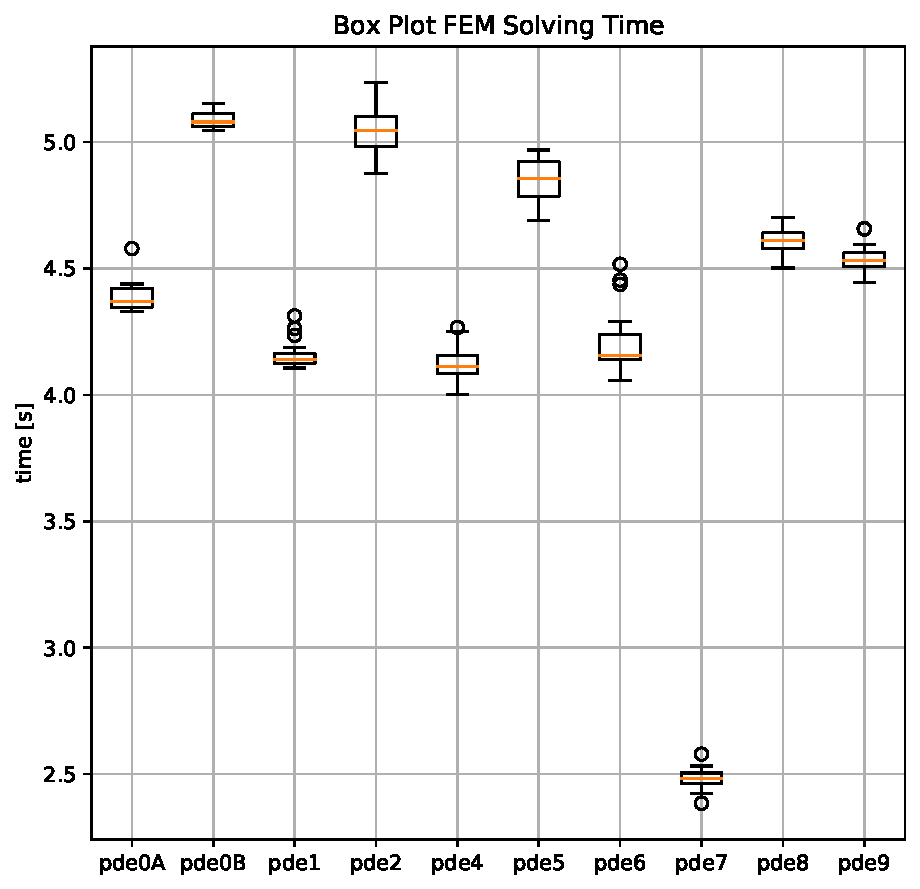
\includegraphics[width=\textwidth]{../../code/experiments/_experiment_fem_base/time_boxplot_pde_0a_0b_1_2_4_5_6_7_8_9.pdf}
	}
	\unterschrift{boxplot: time (in seconds) needed to solve the testbed \gls{pde} (without \gls{pde}3)}{}{}
	\label{fig:_fem_time_boxplot}
\end{figure}

\begin{figure}[H]
	\centering
	\noindent\adjustbox{max width=\linewidth}{
		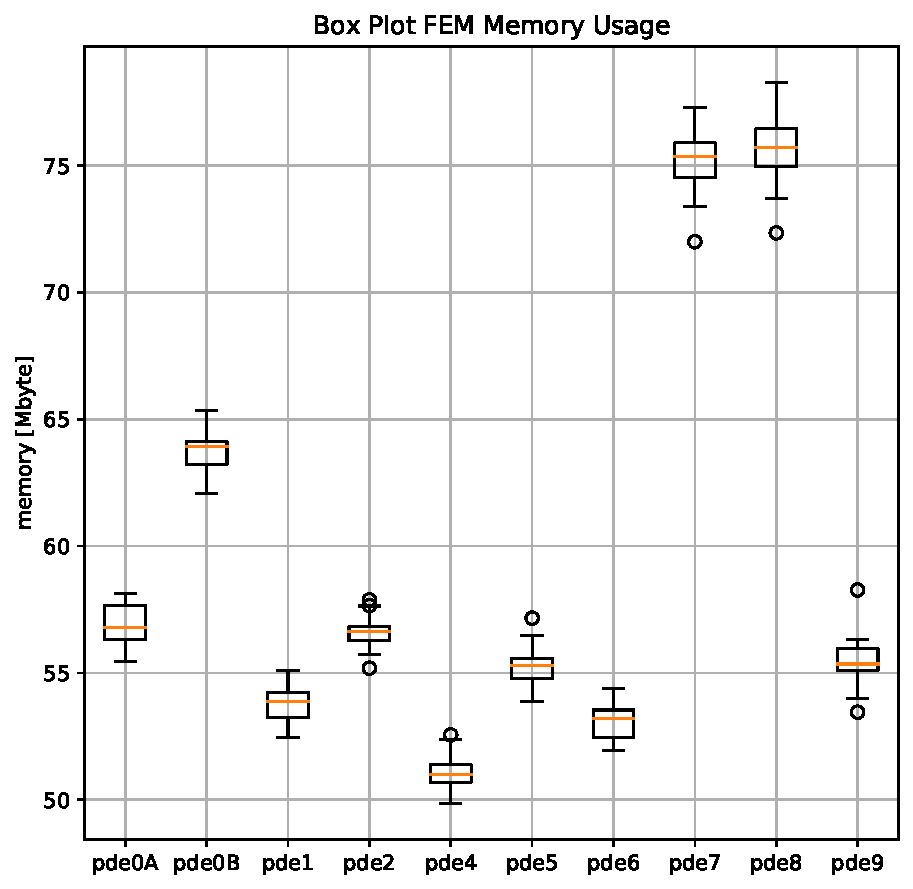
\includegraphics[width=\textwidth]{../../code/experiments/_experiment_fem_base/mem_boxplot_pde_0a_0b_1_2_4_5_6_7_8_9.pdf}
	}
	\unterschrift{boxplot: memory (in Mbyte) needed to solve the testbed \gls{pde} (without \gls{pde}3)}{}{}
	\label{fig:_fem_mem_boxplot}
\end{figure}

\begin{figure}[H]
	\centering
	\noindent\adjustbox{max width=\linewidth}{
		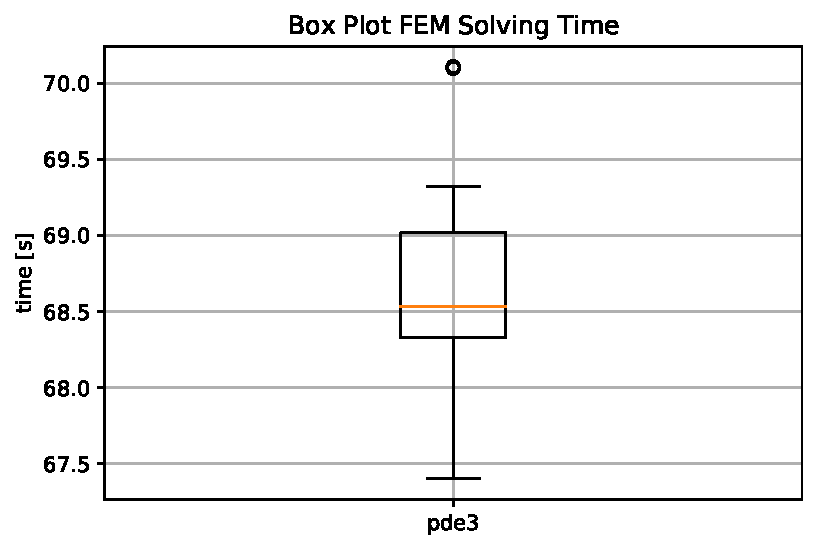
\includegraphics[width=\textwidth]{../../code/experiments/_experiment_fem_base/time_boxplot_pde_3.pdf}
	}
	\unterschrift{boxplot: time to solve testbed \gls{pde}3}{}{}
	\label{fig:_fem_time_boxplot_pde3}
\end{figure}

\begin{figure}[H]
	\centering
	\noindent\adjustbox{max width=\linewidth}{
		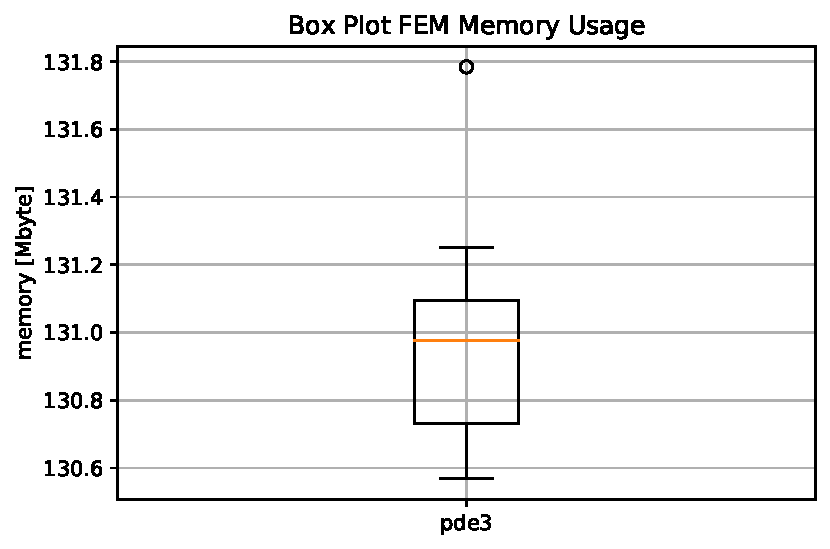
\includegraphics[width=\textwidth]{../../code/experiments/_experiment_fem_base/mem_boxplot_pde_3.pdf}
	}
	\unterschrift{boxplot: memory to solve testbed \gls{pde}3}{}{}
	\label{fig:_fem_mem_boxplot_pde3}
\end{figure}





\end{document}